\subsection{Usage Behavior}
\label{subsec:behavior}

To characterize diurnal user behavior as is observed at the ISP, we first calculate
aggregate data at each time slot, and then plot the median and 90\%-ile of total
usage over a week for both \test and \control sets (Figure~\ref{fig:TS-data-rate-daily}).

We observe that the rise to the peak prime time hour usage on weekdays
is not plateaued like the pattern observed on weekends (and holidays).
A generic (median) weekday aggregate usage consists of a rise in usage that starts
early in the morning that builds up to the prime-time period, peaks, and then falls sharply.
We do not observe a trough in mid afternoon (between 2:00 PM -- 6:00 PM), as is usually
the case for overall usage observed at US Fixed access providers ~\cite{sandvine2014report1}.

\begin{figure}[ht!]
\begin{minipage}{\linewidth}
  \centering
  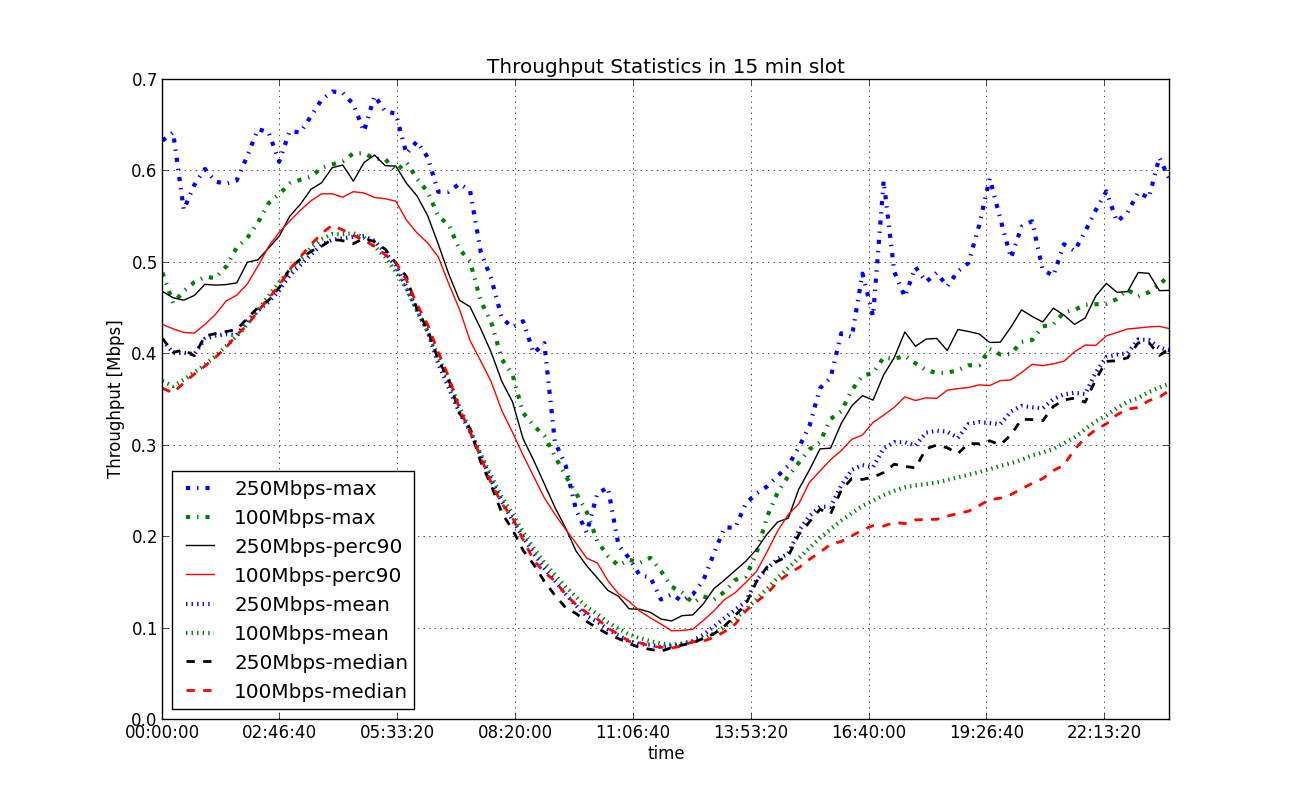
\includegraphics[width=\linewidth]{figures/describe-total-throughput-per-day[replace].png}
  \caption{agg (days) over means (devices): aggregate has no trough, peaks in the evening hours}
  %http://riverside.noise.gatech.edu:8083/separated/full/describe-total-throughput-per-day.png
  \label{fig:TS-data-rate-daily}
\end{minipage}
\end{figure}

To compare the \test and \control sets, we use the average data usage per subscriber
metric (table~\ref{tab:eval-criteria}). We observe that the median prime time and late night
behavior is very similar (7:00 PM -- 7:00 AM), but during off peak usage hours, the \test
set has a higher median than the \control set. This discrepancy occurs completely during the
other half of the day, during work hours. In conclusion, there was no change in
prime time behavior, and an increased usage in off-peak daily hours.

%This lack of troughs could be the result of the users' behavior in higher tier
%bandwidth, and motivated us  to further study user taxonomy in
%section~\ref{subsec:peakratio}.

\todo{see todo.txt for analysis comments}